
%-----------------------------------------------------------------------------------
%	PACKAGES AND OTHER DOCUMENT CONFIGURATIONS
%----------------------------------------------------------------------------------



\documentclass[11pt]{article}

\usepackage[top=2cm, bottom=3cm, left=2cm, right=2cm]{geometry}

\usepackage{apacite}
\setlength{\parindent}{0in}

\newcommand{\Var}{\mathrm{Var}}

\newcommand{\Cov}{\mathrm{Cov}}

\newcommand{\plim}{\rightarrow_{p}}

\usepackage{amsmath, amsfonts}
\usepackage{graphicx}
\usepackage{pdfpages}
\usepackage{bm}
\usepackage{listings}

% Expectation symbol
\newcommand{\E}{\mathrm{E}}
\newcommand{\V}{\mathrm{V}}

%----------------------------------------------------------------------------------
%	TITLE AND AUTHOR(S)
%----------------------------------------------------------------------------------

\title{PubPol 713 Assignment 2} % The article title


\author{Nathan Mather} % The article author(s) 

\date{\today} % An optional date to appear under the author(s)


%----------------------------------------------------------------------------------
\begin{document}
	
%------------------------------------------------------------------------------
%	TABLE OF CONTENTS & LISTS OF FIGURES AND TABLES
%------------------------------------------------------------------------------
\maketitle % Print the title/author/date block

\setcounter{tocdepth}{2} % Set the depth of the table of contents to show sections and subsections only

%\tableofcontents % Print the table of contents

%-------------------------------------------------------------
% Question 1 
%-------------------------------------------------------------
\section{ Question 1}

I generated the variables for a b and c. This is shown in my code in the appendix 


%-------------------------------------------------------------
% Question 2
%-------------------------------------------------------------
\section{ Question 2}

\subsection{A}
I can't seem to figure out how to save tabulate output as a tex file. However, 230,653 individuals are pre-selected and 244,512 are not. Of those scoring below the 475 cutoff, 60.05 are pre-selected, 39.95 are not.  Of those scoring above the cutoff, 43.92 are not pre-selected and 56.08 are pre-Selected. 

The results are summarized in the tables below. 

\begin{center}
	\begin{tabular}{||c | c||} 
		\hline		
		\textbf{pre\_sel}&No.&\% \\
\hline
Not Pre-Selected&244,512.0&51.5 \\
Pre-Selected&230,653.0&48.5 \\
\textbf{Total}&475,165.0&100.0 \\

		\hline
		
	\end{tabular}
\end{center}


\begin{center}
	\begin{tabular}{||c | c | c| c||} 
		\hline
		
		 & \multicolumn{3}{c}{\textbf{pre\_sel}} \\
\textbf{PSU Score Above 475}&\textbf{Not Pre-Selected}&\textbf{Pre-Selected}&\textbf{Total} \\
&\%&\%&\% \\
\hline
Below 475&60.1&39.9&100.0 \\
Above 475&43.9&56.1&100.0 \\
\textbf{Total}&51.5&48.5&100.0 \\

		\hline
		
	\end{tabular}
\end{center}

\subsection{B} 
The normalized score (with a PSU score of 475 equal to 0) has a minimum of -314.5, a max of 375, and a mean of 14.6. The distribution does not seem to show any bunching. A histogram is shown below. 


\begin{center}
	
	\centering
	\textbf{Normalized Test Score period 1 }\par\medskip
	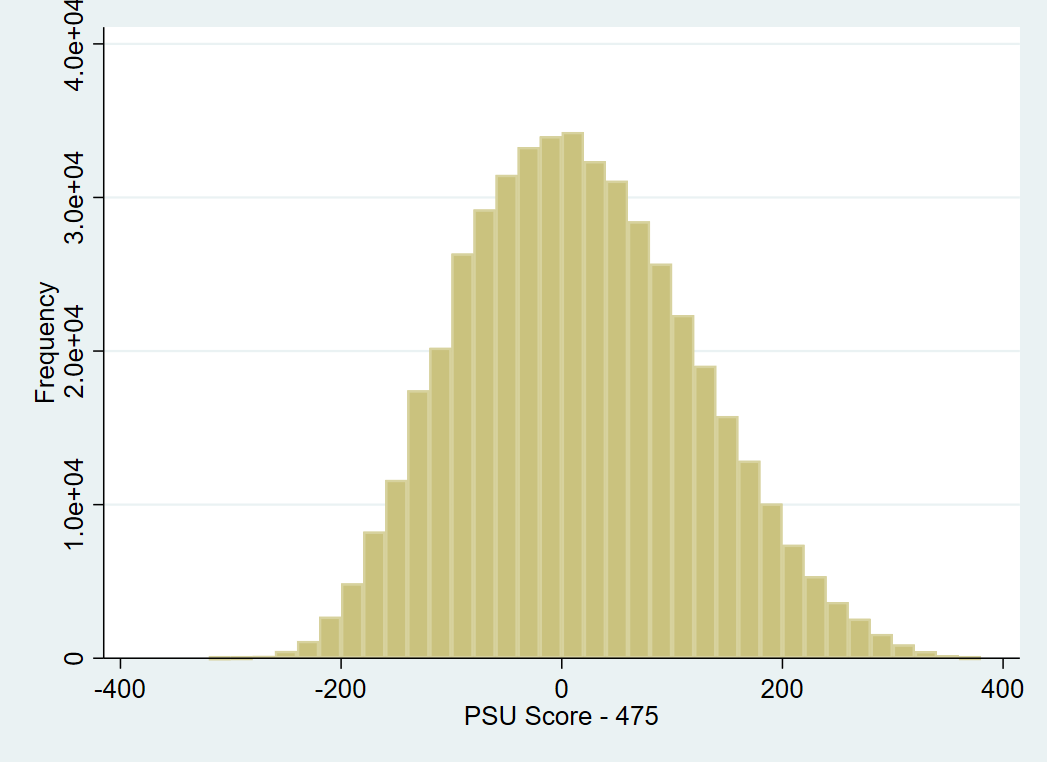
\includegraphics[width=1\linewidth]{2b_hist.png}
\end{center}

\subsection{C } 

The results are summarized in the tables below 

 \begin{center}
 	\begin{tabular}{c | c | c|c} 
 		\hline
 		 & \multicolumn{3}{c}{\textbf{Enrolled in college in t=1}} \\
\textbf{Group}&\textbf{No}&\textbf{Yes}&\textbf{Total} \\
&\%&\%&\% \\
\hline
Not Pre-Sel&74.4&25.6&100.0 \\
Pre-Sel Below&88.9&11.1&100.0 \\
Pre-Sel Above&36.3&63.7&100.0 \\
\textbf{Total}&65.7&34.3&100.0 \\

 		\hline
 		
 	\end{tabular}
 \end{center}
 

 \begin{center}
	\begin{tabular}{c | c | c|c} 
		\hline
		 & \multicolumn{3}{c}{\textbf{Ever enrolled flag}} \\
\textbf{Group}&\textbf{No}&\textbf{Yes}&\textbf{Total} \\
&\%&\%&\% \\
\hline
Not Pre-Sel&62.2&37.8&100.0 \\
Pre-Sel Below&80.1&19.9&100.0 \\
Pre-Sel Above&25.5&74.5&100.0 \\
\textbf{Total}&54.5&45.5&100.0 \\

		\hline
		
	\end{tabular}
\end{center}


\subsection{D } 

The results are summarized in the tables below 

\begin{center}
	\begin{tabular}{c | c | c|c} 
		\hline
		 & \multicolumn{3}{c}{\textbf{Enrolled in college in t=1}} \\
\textbf{Income quintile for year 1}&\textbf{No}&\textbf{Yes}&\textbf{Total} \\
&\%&\%&\% \\
\hline
1&64.7&35.3&100.0 \\
2&54.3&45.7&100.0 \\
3&47.7&52.3&100.0 \\
4&43.0&57.0&100.0 \\
5&51.2&48.8&100.0 \\
\textbf{Total}&55.8&44.2&100.0 \\

		\hline
		
	\end{tabular}
\end{center}


\begin{center}
	\begin{tabular}{c | c | c|c} 
		\hline
		 & \multicolumn{3}{c}{\textbf{Ever enrolled flag}} \\
\textbf{Income quintile for year 1}&\textbf{No}&\textbf{Yes}&\textbf{Total} \\
&\%&\%&\% \\
\hline
1&56.4&43.6&100.0 \\
2&44.4&55.6&100.0 \\
3&35.9&64.1&100.0 \\
4&29.7&70.3&100.0 \\
5&31.3&68.7&100.0 \\
\textbf{Total}&44.7&55.3&100.0 \\

		\hline
		
	\end{tabular}
\end{center}




%-------------------------------------------------------------
% Question 3
%-------------------------------------------------------------
\section{ Question 3}

Below is a table showing the distribution of PSU scores by income quantile. There is also a verticle line at zero indicating the point to look for discontinuities. The distributions all appear to change smoothly across zero. 


 	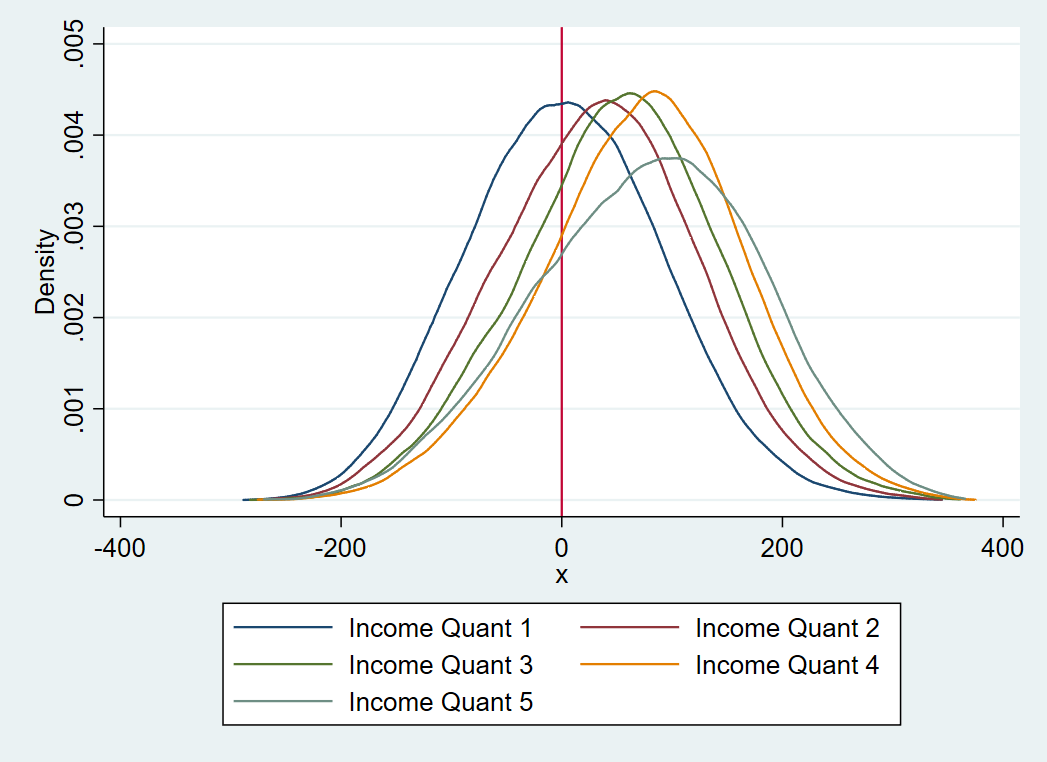
\includegraphics[width=1\linewidth]{3_plot.png}


%-------------------------------------------------------------
% Question 4
%-------------------------------------------------------------
\section{ Question 4}

Below I have the results from table three of the paper replicated. I used the same regression equation and bandwidth of 44. The main coefficient of interest here is the ``PSU score Above 475". In column 1 this coefficient shows that, for pre-selected students, being above the cutoff implies an increase of 17.5 percentage points in the probability of enrolling in college immediately after the test. One potential threat to interpreting this relationship as causal is that passing the 475 threshold may provide some benefit other than loan eligibility. An example discussed in the paper is higher probability of acceptance to schools if students score above 475. Column two tests this possibility with a placebo test on non-selected students. Here be find no significant effect for being above the 475 mark. This is what we would expect since these students are not eligible for loans anyway. 

\begin{center}
	\textbf{Table 3 Replication}\par\medskip
		{
\def\sym#1{\ifmmode^{#1}\else\(^{#1}\)\fi}
\begin{tabular}{l*{2}{c}}
\hline\hline
                    &\multicolumn{1}{c}{(1)}&\multicolumn{1}{c}{(2)}\\
\hline
PSU Score Above 475 &       0.175\sym{***}&     0.00273         \\
                    &   (0.00611)         &   (0.00556)         \\
[1em]
PSU Score - 475     &     0.00160\sym{***}&     0.00163\sym{***}\\
                    &  (0.000147)         &  (0.000133)         \\
[1em]
PSU Score if Above 475&     0.00222\sym{***}&    0.000866\sym{***}\\
                    &  (0.000238)         &  (0.000223)         \\
[1em]
Constant            &       0.182\sym{***}&       0.159\sym{***}\\
                    &   (0.00387)         &   (0.00367)         \\
\hline
Bandwidth           &          44         &          44         \\
\hline\hline
\multicolumn{3}{l}{\footnotesize Standard errors in parentheses}\\
\multicolumn{3}{l}{\footnotesize \sym{*} \(p<0.05\), \sym{**} \(p<0.01\), \sym{***} \(p<0.001\)}\\
\end{tabular}
}


\end{center}


In addition to the straight replication, I also ran these regressions using an updated bandwidth selection technique and local linear regression  \cite{matias_14}. The results are similar and can be found in the table below. ``RD\_Estimate" is comparable to ``PSU Score Above 475" in the table above. 


\begin{center}
		\textbf{Table 3 with updated methods}\par\medskip
	{
\def\sym#1{\ifmmode^{#1}\else\(^{#1}\)\fi}
\begin{tabular}{l*{2}{c}}
\hline\hline
                    &\multicolumn{1}{c}{(1b)}&\multicolumn{1}{c}{(2b)}\\
\hline
RD\_Estimate         &       0.176\sym{***}&     0.00281         \\
                    &   (0.00668)         &   (0.00569)         \\
\hline
Bandwidth           &       44.61         &       50.29         \\
\hline\hline
\multicolumn{3}{l}{\footnotesize Standard errors in parentheses}\\
\multicolumn{3}{l}{\footnotesize \sym{*} \(p<0.05\), \sym{**} \(p<0.01\), \sym{***} \(p<0.001\)}\\
\end{tabular}
}

	
\end{center}
%------------------------------------------------------------------------------
% bib
%------------------------------------------------------------------------------
\bibliographystyle{apacite}
\bibliography{References}


%-----------------------------------------------
% end doc
%------------------------------------------------
\end{document}


